\documentclass[11pt,a4paper]{article}
\usepackage[T1]{fontenc}
\usepackage[utf8]{inputenc}
\usepackage{lmodern,microtype}
\usepackage{amsmath,amssymb,amsthm,mathtools,bm}
\usepackage{booktabs,array,longtable,graphicx,float,xcolor}
\usepackage[margin=2.05cm]{geometry}
\usepackage{enumitem,fancyhdr,hyperref}
\hypersetup{unicode=true,colorlinks=true,linkcolor=blue!45!black,urlcolor=blue!55!black,
 pdftitle={FIN ST417--ST431: Global Gain Enclosure, Singular IR Attachment, and a Local Morse Atlas},
 pdfauthor={Krzysztof Żuchowski},
 pdfsubject={Local analytical and computational continuation of FIN},
 pdfkeywords={FIN, strict kernel, gain transition, Krawczyk, singular continuation, Morse theory, invariant theory, Chernoff transfer}}
\pagestyle{fancy}\fancyhf{}\lhead{FIN ST417--ST431}\rhead{Release 10.85}\cfoot{\thepage}
\setlength{\headheight}{14pt}
\newcommand{\Proven}{\textcolor{green!38!black}{\textbf{[PROVEN]}}}
\newcommand{\Evidence}{\textcolor{orange!80!black}{\textbf{[STRONG NUMERICAL EVIDENCE]}}}
\newcommand{\Partial}{\textcolor{orange!80!black}{\textbf{[PARTIAL]}}}
\newcommand{\Blocked}{\textcolor{red!65!black}{\textbf{[BLOCKED]}}}
\newtheorem{theorem}{Theorem}
\newtheorem{proposition}{Proposition}
\newtheorem{corollary}{Corollary}

\title{\textbf{FIN ST417--ST431}\\[3pt]
Global Gain Enclosure, Singular Infrared Attachment,\\
and a Locally Certified Morse Atlas\\[6pt]
\large Release 10.85}
\author{Krzysztof \.{Z}uchowski\\
\small Independent Researcher --- Fractal Information Theory Project\\
\small ORCID: 0009-0002-0909-3613}
\date{14 August 2026}

\begin{document}
\maketitle

\begin{abstract}
Programs ST417--ST431 continue the finite analytical and computational FIN
program after Release 10.84.  Three results materially sharpen the mathematical
state map.  First, an entropy--collision extremal reduction and an outward
spectral enclosure prove that the uniform probability is the unique global
minimum of the supplied strict functional for
$0\le g\le2.251344001799089$.  Together with the certified localized orbit near
$g=4$, the first global orbit change is enclosed in
$[2.251344001799089,3.999]$.  The known branch-local coexistence value
$2.90249648\ldots$ is not promoted to the global critical gain.

Second, the singular continuum-IR limit is regularized by
$b=1/y_3$ and $c=a y_3$.  A single parametric Krawczyk box covers every
$b\in[0,0.002]$, including the flat $b=0$ extension.  This proves that the
finite upper-band branch attaches uniquely to the compactified face
$y_3=\infty$, $a=0$; the attachment is no longer merely numerical.  Third,
all nine stationary $D_{12}$-orbit representatives previously found at $g=4$
are locally isolated by interval arithmetic, with certified Morse-index
histogram $2$ minima, $4$ index-one saddles, and $3$ index-two saddles.  The
atlas is local and nonexhaustive.

The batch also doubles the certified localized-gain tube to
$[3.998,4.002]$, constructs a joint odd/even modular generator census through
degree six, improves a synthetic sextic design condition number by a factor
$1.254$, and compares a rigorous Chernoff cone bound with stable finite-grid
spectra.  An attempt to compute 136 explicit degree-eight syzygies exceeded a
declared local resource stop and produced no basis.  No result derives the
gain, selects one symmetry-broken orbit member, supplies dimensional units,
completes the legacy-to-strict bridge, or adds independent empirical evidence.
\end{abstract}

\tableofcontents
\newpage

\section{Scope, audited object, and epistemic boundary}

The repository baseline is Git commit
\texttt{bb540a767e210a5a3bf816e4868e7bcefbac3872}, supplemented by the
local ST402--ST416 packet and the executable artifacts of this release.  The
strict finite operator is
\begin{equation}\label{eq:A}
 A=sI-W,\qquad W_{xx}=0,\qquad
 W_{xy}=\frac{\cos(0.18575\,d(x,y)+0.16250)}{1+d(x,y)^{9/5}}quad(x\ne y),
\end{equation}
on $\mathbb Z_{12}$, with off-diagonal row sum
$s=1.660307278766099\ldots$.  The supplied variational family is
\begin{equation}\label{eq:V}
 V_g(p)=D(p\Vert u)-\frac g2(p-u)^TA(p-u),\qquad
 D(p\Vert u)=\sum_{i=0}^{11}p_i\log(12p_i),\qquad u_i=\frac1{12}.
\end{equation}
All quantities in this report are dimensionless.

The legacy ontological kernel remains an intermediate bridge kernel.  It is
not silently substituted for \eqref{eq:A}, and no historical electroweak,
electromagnetic, gravitational, Planck-scale, or dimensional role is
transferred to the strict kernel.  The project ontology---the nadsoliton itself
as primordial fractal information in a solitonic state, followed internally by
light, matter, and an emergent observer---is retained as context.  It is not a
premise in the finite proofs below.

An orbit of twelve minima is not a selector.  QW-2191 remains open.  A theorem
conditional on $g$ does not generate $g$.  A dimensionless optimization
boundary is not a laboratory phase transition.  Local computation is not
external validation.

\section{Executive result ledger}
\small
\begin{longtable}{>{\raggedright\arraybackslash}p{.075\textwidth}>{\raggedright\arraybackslash}p{.19\textwidth}>{\raggedright\arraybackslash}p{.63\textwidth}}
\toprule Program&Status&Result\\\midrule\endhead
ST417&\Blocked&The exact lower bound of 136 degree-eight relations survives, but Singular produced no explicit basis within the declared local stop.\\
ST418&\Proven&The unique uniform-global regime extends through $g=2.251344001799089$; the first global orbit change lies in $[2.251344001799089,3.999]$.\\
ST419&\Proven&A one-sided parametric Krawczyk theorem proves unique attachment of the finite continuum-IR branch to the compactified $a=0$, $y_3=\infty$ face.\\
ST420&\Proven&Exactly twelve global minima, one $D_{12}$ orbit, persist uniformly for every $g\in[3.998,4.002]$.\\
ST421&\Proven{} local&Nine stationary-orbit representatives and their Morse indices are interval-certified; completeness remains open.\\
ST422&\Evidence&Replicator-gradient integrations give a numerical barrier graph from the four certified index-one saddles.\\
ST423&\Partial&Finite-root and singular-root tubes are certified, but no full enlarged complement-sign topology cover was obtained.\\
ST424&\Proven{} modular&A joint odd/even quotient census through degree six gives primitive counts $(6,12,32,52,55)$ in degrees $2$--$6$ over the declared finite field.\\
ST425&\Evidence&A pivoted synthetic 500-row design improves sextic conditioning by a factor $1.254$ relative to a same-pool random design.\\
ST426&\Proven{} bound / \Evidence{} spectrum&The cone contraction upper bound remains rigorous; three Ulam grids give stable but noncertified spectral ratios near $0.5958$.\\
ST427&\Proven{} conditional&A small nonlinear basin has a paid input-to-state stability inequality under bounded tangent forcing.\\
ST428&\Blocked&Mixed signs in the rank-seven mediator prevent transfer of the strict positive-weight global envelope.\\
ST429&\Blocked&No new strict typed source of the nonzero gain is exported.\\
ST430&\Blocked&No new nonpremise selector or orientation provider is exported; QW-2191 remains open.\\
ST431&\Blocked&No independent referee, laboratory record, held-out custody, or empirical datum is added.\\
\bottomrule
\end{longtable}
\normalsize

\section{ST418: a rigorous global gain-transition enclosure}

Put $q=p-u$ and $r=\lVert q\rVert_2^2$.  The entropy maximizer at fixed
collision has one large coordinate and eleven equal smaller coordinates,
\begin{equation}\label{eq:Dmin}
 a=\frac{1+\sqrt{132r}}{12},\qquad b=\frac{1-a}{11},\qquad
 D_{\min}(r)=a\log(12a)+11b\log(12b).
\end{equation}
For completeness, the code covers every two-level Lagrange branch: if the
large value has multiplicity $k$, then
\[
 a_k=\frac1{12}+\sqrt{\frac{(12-k)r}{12k}},\qquad
 b_k=\frac1{12}-\sqrt{\frac{kr}{12(12-k)}}.
\]
The stationarity equation $\log p+\alpha+\beta p=0$ has at most two positive
roots.  Smoothing/majorization singles out the $k=1$ branch as the entropy
maximum; boundary faces are bounded by its smoothing limits.  A 46,200-cell
outward cover, with a Hessian bound near $r=0$ and an analytic endpoint bound,
gives
\begin{equation}\label{eq:c}
 D(p\Vert u)\ge c\lVert p-u\rVert_2^2,qquad
 c\ge2.636528744728136.
\end{equation}

Because \eqref{eq:A} is circulant, its eigenvalues are directly enclosed by
\[
 \lambda_k=s-2\sum_{d=1}^{5}w_d\cos(2\pi kd/12)-w_6(-1)^k.
\]
Outward arithmetic gives
\[
 \lambda_{\max}(A)\le2.342182041146301.
\]
Combining this with \eqref{eq:c},
\[
 V_g(p)\ge\left(c-\frac{g\lambda_{\max}}2\right)\lVert p-u\rVert_2^2.
\]

\begin{theorem}[Certified uniform-global regime]
For every supplied dimensionless gain
\[
 0\le g\le2.251344001799089,
\]
$u$ is the unique global minimizer of \eqref{eq:V}.
\end{theorem}

Release 10.84 proves a nonuniform twelve-point global orbit for every
$g\in[3.999,4.001]$.  Therefore a first global orbit change exists in
\begin{equation}\label{eq:transition}
 [2.251344001799089,3.999].
\end{equation}
The branch-local equal-value point $2.90249648\ldots$ lies inside
\eqref{eq:transition}, but no global exhaustion theorem has yet isolated it.
It remains incorrect to call that number the global critical gain.

\begin{figure}[H]\centering
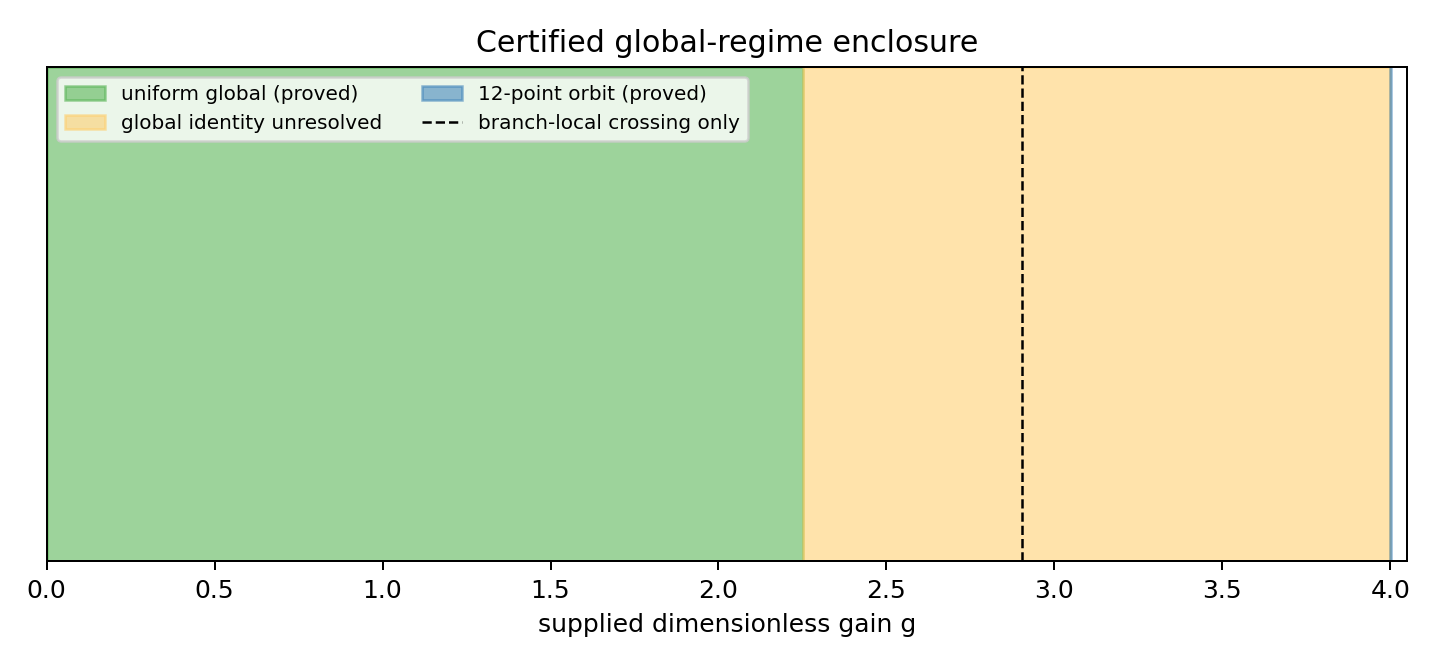
\includegraphics[width=.88\textwidth]{FIN_ST417_ST431_Figures/gain_enclosure.png}
\caption{What is proved and what remains unresolved in the supplied gain family.}
\end{figure}

\section{ST419: singular attachment of the continuum-IR branch}

The original KKT system has three thresholds $0<y_1<y_2<y_3$, mixing
coefficient $a$, multiplier $\nu$, active time $T$, budget $3$, and stationarity
function
\begin{equation}\label{eq:G}
 G(y)=\frac{2ay}{1+e^{-y}}+
 \frac{2T(1-a)y e^{-(T-1)y}}{1+e^{-Ty}}-\nu.
\end{equation}
ST415 certified a limiting four-equation face at $a=0$, $y_3=\infty$, but did
not certify that the finite branch reaches it.

Introduce
\begin{equation}\label{eq:compact}
 b=\frac1{y_3},\qquad c=ay_3,\qquad a=bc.
\end{equation}
The third stationarity equation becomes
\[
 \frac{2c}{1+e^{-1/b}}+
 \frac{2T(1-bc)b^{-1}e^{-(T-1)/b}}{1+e^{-T/b}}-\nu=0.
\]
The functions $e^{-1/b}$, $b e^{-1/b}$, and
$b^{-1}e^{-(T-1)/b}$ admit zero-valued $C^\infty$ extensions at $b=0$.
The budget tail obeys
$0\le E_1(1/b)\le b e^{-1/b}$; analogous explicit exponential bounds pay
the integral tail and every Jacobian tail.

A common Krawczyk box, centered at the $b=0.001$ root, uses radii
\[
 (1.6\!\times\!10^{-7},1.05\!\times\!10^{-3},2.1\!\times\!10^{-5},
 4.2\!\times\!10^{-5},1.55\!\times\!10^{-3})
\]
for $(y_1,y_2,c,\nu,T)$.  Its smallest inclusion margin is
$2.3433822\times10^{-8}$ on the full parameter interval $b\in[0,0.002]$.

\begin{theorem}[One-sided singular attachment]
For each $b\in[0,0.002]$, the regularized five-equation system has exactly one
root in the common interval box.  For $b>0$ it is a root of the original
finite-$y_3$ KKT equations.  At $b=0$ it equals the unique ST415 limiting-face
root.  Hence the finite upper-band branch attaches continuously and uniquely
to the compactified face, with $y_3\to\infty$ and $a\to0$.
\end{theorem}

This proves an optimization-theoretic attachment.  It does not create a
physical infrared scale, dimensional wavelength, or experimental phase.

\begin{figure}[H]\centering
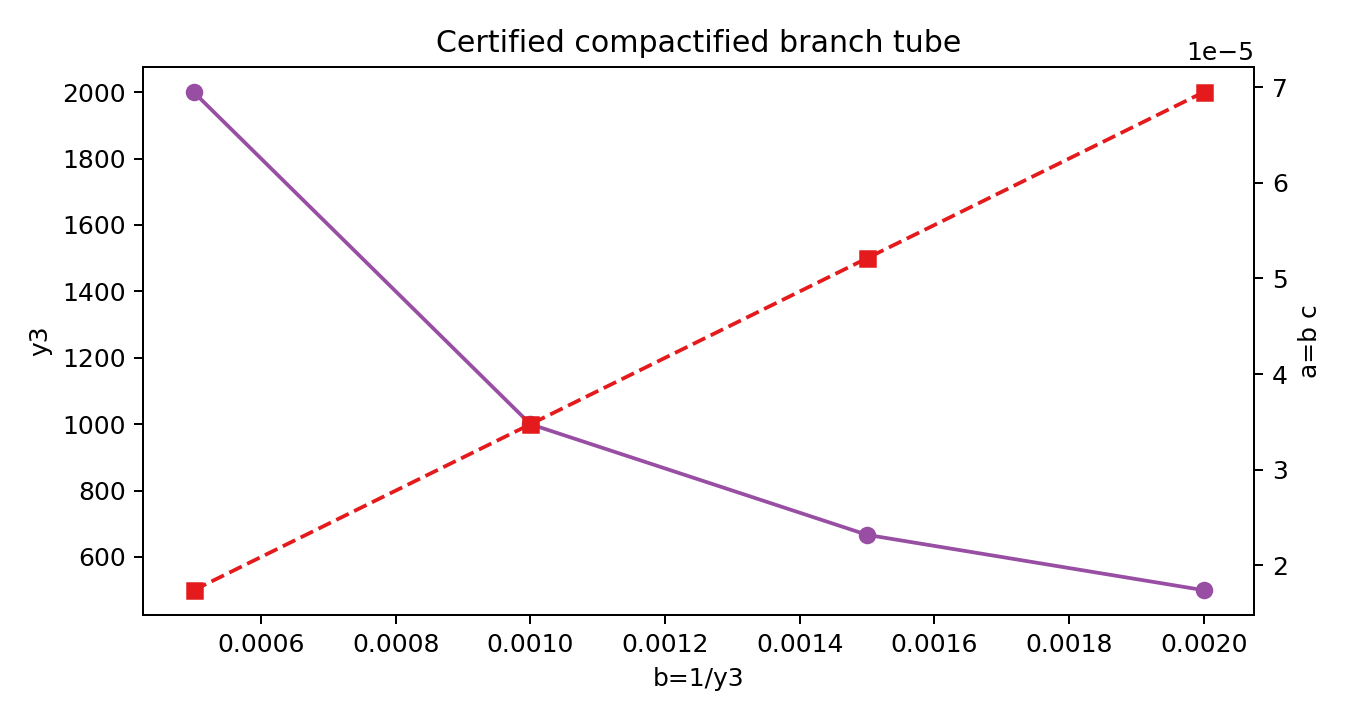
\includegraphics[width=.78\textwidth]{FIN_ST417_ST431_Figures/ir_attachment.png}
\caption{Replay points inside the certified compactified branch tube.  The theorem is the interval box, not the plotted samples.}
\end{figure}

\section{ST420: doubled persistence tube near supplied gain four}

The Release 10.84 orbit-exhaustion argument is replayed with 20,000 collision
cells.  A common rational $g=4$ benchmark and cap threshold $p_i>0.94$ give
\[
 \inf_{\max p_i\le0.94}
 \bigl(V_{3.998}(p)-V_{3.998}(p_{\rm rat})\bigr)
 \ge1.8111997969\times10^{-4}.
\]
The benchmark quadratic exceeds the outside energy upper bound by
$0.0663087333\ldots$, paying the monotonicity step.  At the other endpoint,
the worst Euclidean cap-curvature margin is $0.3079009418\ldots>0$.

\begin{corollary}
For every $g\in[3.998,4.002]$, the global minimizer set of \eqref{eq:V}
consists of exactly twelve points in one $D_{12}$ orbit.
\end{corollary}

The half-width is twice that of ST405.  It remains a local persistence result;
it does not approach the lower end of \eqref{eq:transition}.

\section{ST421--ST422: local Morse atlas and barrier evidence}

Interior stationarity is written without softmax coordinates:
\begin{equation}\label{eq:stat}
 \log(12p_i)+1-4(Ap)_i+\lambda=0,qquad \sum_i p_i=1.
\end{equation}
Each of the nine previously sampled orbit representatives is refined as a
thirteen-variable root $(p,\lambda)$.  A radius-$2\times10^{-9}$ interval box
around each root satisfies strict Krawczyk inclusion.  The smallest of all nine
inclusion margins is $1.99946\times10^{-9}$.  Perturbation bounds for
$\operatorname{diag}(1/p_i)-4A$ separate every tangent eigenvalue from zero.

\begin{proposition}[Locally certified atlas]
The nine supplied representatives are locally unique stationary roots of
\eqref{eq:stat}.  Their certified Morse-index histogram is
\[
 \#\operatorname{index}0=2,qquad
 \#\operatorname{index}1=4,qquad
 \#\operatorname{index}2=3.
\]
\end{proposition}

This proposition does not prove that nine is the complete orbit count.  That
would require an interval cover of the entire eleven-simplex modulo symmetry.

For a qualitative barrier graph, ST422 integrates the simplex-preserving
replicator gradient flow
\[
 \dot p_i=-p_i\bigl(\partial_iV_4-\langle p,\nabla V_4\rangle\bigr)
\]
from both sides of each certified index-one saddle.  One saddle connects the
uniform minimum to a localized minimum numerically; the other three descend
to different translates of the localized orbit.  Endpoint distances lie
between $1.5\times10^{-12}$ and $5.4\times10^{-11}$.  These are deterministic
finite-time integrations, not certified heteroclinic or Conley-index results.

\begin{figure}[H]\centering
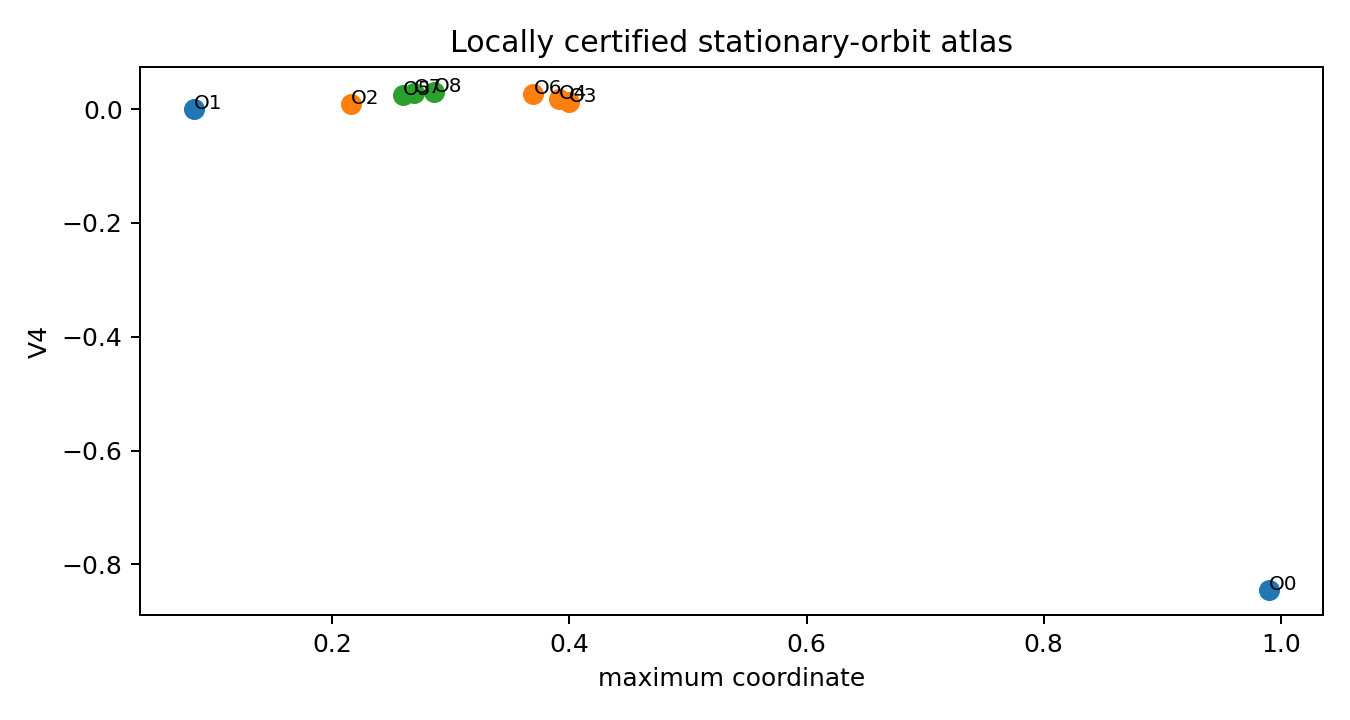
\includegraphics[width=.78\textwidth]{FIN_ST417_ST431_Figures/stationary_atlas.png}
\caption{The nine locally certified stationary representatives.  Absence of additional orbits is not proved.}
\end{figure}

\section{ST417 and ST424: invariant algebra---advance and failure}

\subsection{Degree-eight syzygy attempt}

The declared even generator family contains six quadratics, $32$ primitive
quartics, and $117$ primitive sextics.  Its formal degree-eight products are
\[
 \binom94=126,qquad \binom72\,32=672,qquad
 \binom{33}{2}=528,qquad 6\cdot117=702,
\]
for a total of $2028$.  Since the degree-eight invariant space has dimension
$1892$, at least $136$ relations are forced.

ST417 constructed the complete $1892\times2028$ evaluation matrix over
$\mathbb F_{1000003}$.  Both \texttt{syz(M)} and \texttt{rank(M)} in locally
available Singular exceeded the declared 60-second stop and were interrupted
without output.  No relation vector was retained.  Therefore the exact lower
bound $136$ survives, but an explicit basis was not computed.  Even a modular
basis would still require multi-prime lifting and direct characteristic-zero
identity verification before promotion to integral syzygies.

\subsection{Odd generators change the census}

The earlier presentation was even-only.  ST424 includes odd invariants and
uses exact modular pivots on the mean-zero hyperplane.  There are twelve
primitive cubic directions.  At degree five, the $72$ products quadratic
times cubic have rank $72$, leaving $52$ primitive modular quotient
directions.  At degree six, the joint family
\[
 q^3,\qquad q\,p_4,\qquad p_3^2
\]
has $326$ formal products and modular rank $310$, leaving $55$ selected
primitive completion directions.  The resulting modular primitive census is
\[
 \begin{array}{c|ccccc}
 \text{degree}&2&3&4&5&6\\\hline
 \text{primitive quotient count}&6&12&32&52&55.
 \end{array}
\]
This is a joint finite-field quotient certificate through degree six, not yet
a minimal characteristic-zero ring presentation through degree eight.

\begin{figure}[H]\centering
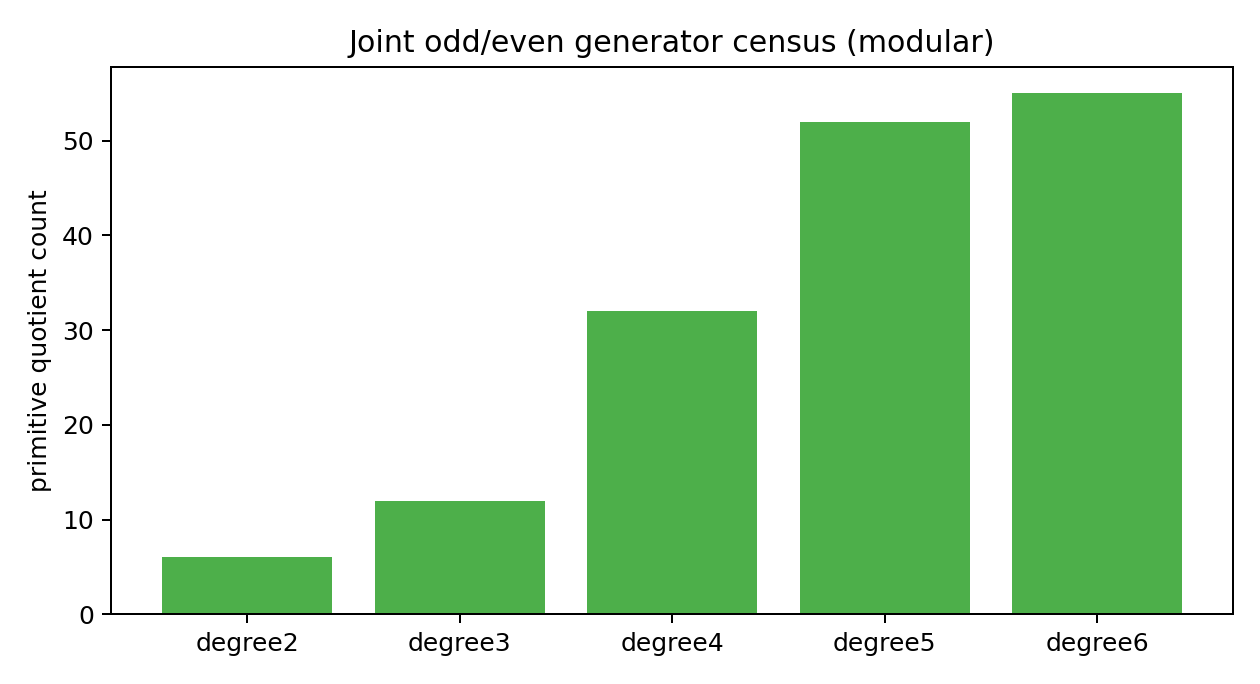
\includegraphics[width=.72\textwidth]{FIN_ST417_ST431_Figures/invariant_census.png}
\caption{Joint odd/even modular primitive quotient counts through degree six.}
\end{figure}

\section{ST425--ST428: design, transfer, robustness, and rank seven}

\subsection{Synthetic invariant design}

From a pool of $1800$ mean-zero unit vectors, pivoted QR selects $500$ rows for
the complete $365$-coefficient sextic design.  After column normalization,
the selected design has condition number $14965.05$, versus $18764.64$ for a
same-pool random design, an improvement factor $1.2539$.  This remains
ill-conditioned and wholly synthetic.  It is an algorithmic design result,
not a detector or laboratory calibration.

\subsection{Chernoff transfer sharpness}

The rigorous adapted-cone result gives contraction at most
$0.9800737084\ldots$.  Bilinear Ulam discretizations on $21^2$, $31^2$, and
$41^2$ belief-pair grids give leading eigenvalues near $0.48202$ and
second-to-first modulus ratios
\[
 0.595845,qquad0.595826,qquad0.595751.
\]
Their stability shows that the analytic cone bound is conservative.  It does
not provide an interval lower bound on the infinite-dimensional spectral gap,
and the HMM fixture remains supplied rather than FIN-derived.

\subsection{Nonlinear local forcing}

At a localized minimum, the smallest tangent Hessian eigenvalue at the center
is $86.33235\ldots$.  On a radius-$10^{-6}$ ball, the paid diagonal-Hessian
variation is at most $21.90150\ldots$, leaving
$\mu\ge64.43086$.  If a tangent perturbation has norm at most $\epsilon$, then
while the trajectory stays in this ball,
\[
 \lVert e(t)\rVert\le e^{-\mu t}\lVert e(0)\rVert+
 \frac{\epsilon}{\mu}(1-e^{-\mu t}).
\]
For $\lVert e(0)\rVert<R/2$ and
$\epsilon<\mu R/2=3.2215\times10^{-5}$, the ball is invariant.  Time and
forcing here are dimensionless supplied objects.

\subsection{Why rank seven still does not inherit the global theorem}

The rank-seven mediator shares the seven positive eigenvalues of the strict
operator, including $\lambda_{\max}=2.3421820411\ldots$, but its off-diagonal
entries have $24$ positive and $42$ negative pairs.  The positive-weight
collision envelope used for the strict Laplacian therefore cannot be
transferred.  A sign split is valid but does not close the global gap.  Equal
spectra do not imply equal positivity geometry.

\section{Falsification ledger and surviving interpretation}

\begin{itemize}[leftmargin=1.5em]
\item \textbf{Global transition.}  A nonzero lower endpoint is proved, but
neither uniqueness nor the value of the transition is proved.  The local
crossing is explicitly not promoted.
\item \textbf{IR boundary.}  The singular attachment is now proved in one
common tube.  A full enlarged complement-sign topology cover remains absent.
\item \textbf{Morse landscape.}  Nine roots and indices are locally proved.
The number nine is not globally exhaustive; heteroclinic edges are numerical.
\item \textbf{Invariant algebra.}  The odd/even degree-six modular census is
new.  The explicit degree-eight relation basis failed under the resource stop.
\item \textbf{Dynamics.}  A local forced-flow inequality is proved under a
declared dimensionless flow.  It does not derive a physical clock or bath.
\item \textbf{Physical bridge.}  No source for $g$, selector, dimensional
calibration, preparation, instrument, environment, apparatus, or record was
generated.
\end{itemize}

The deepest conclusion that survives this batch is mathematical rather than
ontological: the supplied strict finite spectral object supports a rigorously
controlled entropy--quadratic phase family, a compactifiable singular
optimization branch, and a nontrivial invariant algebra.  These structures
are mutually compatible, but they do not yet form a theorem deriving
experimentally testable physics from primordial information.

\section{Recommended programs ST432--ST446}

\begin{longtable}{>{\raggedright\arraybackslash}p{.08\textwidth}>{\raggedright\arraybackslash}p{.53\textwidth}>{\raggedright\arraybackslash}p{.12\textwidth}>{\raggedright\arraybackslash}p{.17\textwidth}}
\toprule Program&Acceptance test&Priority&Expected status\\\midrule\endhead
ST432&Compute a sparse degree-eight modular kernel with durable checkpoints; lift across at least two primes and verify every retained relation directly over the integers.  Reject a merely floating nullspace.&1&Hard exact algebra\\
ST433&Construct an interval branch-and-bound lower bound for $V_g$ on the entire simplex over successive gain slabs inside $[2.2513440,3.998]$.  Each slab must identify all admissible global orbit types.&1&High-value proof\\
ST434&If ST433 isolates one crossing, certify equality of the competing branch values, transversality, and absence of a third competitor.  This is the acceptance gate for a unique global critical gain.&1&Conditional on ST433\\
ST435&Cover a $D_{12}$ fundamental domain of the eleven-simplex with interval Newton/Krawczyk boxes and exclusion boxes.  Accept only if the nine-orbit stationary atlas is exhaustive.&1&Computationally hard\\
ST436&Replace the ST422 integrations by isolating blocks or a Conley/Morse connection certificate for at least the uniform-to-localized index-one saddle.&2&Topological proof\\
ST437&Maximize the certified singular-attachment interval in $b$ using adaptive parameter subdivision and prove where the common branch tube first fails or folds.&2&Likely feasible\\
ST438&Produce the missing complement-sign cover for the enlarged continuum-IR rectangle, including root ordering, derivative signs, inactive slack, and tail exclusion.&2&Proof-grade topology\\
ST439&Lift the joint odd/even generator census to characteristic zero and compute a minimal presentation through degree eight, including relations rather than only quotient counts.&2&Hard exact algebra\\
ST440&Optimize the sextic design for the smallest singular value under bounded observation noise; compare D-, E-, and minimax designs on a frozen candidate pool and hold-out pool.&3&Numerical design\\
ST441&Build a collectively compact finite-rank approximation of the synthetic Chernoff transfer with explicit discretization error, giving certified upper and lower spectral-gap brackets.&2&Functional analysis\\
ST442&Seek a global or cap-scale Lyapunov basin for the localized orbit under bounded tangent forcing, with positivity and simplex-boundary control.&3&Nonlinear dynamics\\
ST443&Formulate a sign-aware SDP or copositive relaxation for the rank-seven mediator and accept it only if the global value bound overlaps a certified feasible root.&3&Operator optimization\\
ST444&Reopen gain sourcing only if a genuinely new strict typed scalar source or normalization law appears; otherwise preserve ST429 without replay.&Gate&Source dependent\\
ST445&Reopen selector/orientation only if a new nonpremise strict provider escapes the exhausted $D_{12}$-invariant class; otherwise preserve QW-2191.&Gate&Provider dependent\\
ST446&Accept physical promotion only after independent preparation, calibrated clock, vertex-resolving instrument, raw event record, frozen hold-out, and separated custody are supplied.&Gate&External evidence\\
\bottomrule
\end{longtable}

The recommended execution order is
\[
 \boxed{\text{ST433}\rightarrow\text{ST434},\qquad
        \text{ST432}\rightarrow\text{ST439},\qquad
        \text{ST437}\rightarrow\text{ST438},\qquad
        \text{ST435}\rightarrow\text{ST436}.}
\]
ST444--ST446 are event-driven gates, not invitations to repeat closed searches.

\section{Reproducibility and provenance}

The executable entry point is
\texttt{fin\_st417\_st431\_research.py}.  It emits one aggregate JSON, fifteen
program packets, one CSV ledger, and four figures.  The independent test suite
\texttt{test\_fin\_st417\_st431.py} contains nineteen tests covering live matrix
properties, the regularized face residual, stationary residuals, packet hashes,
interval-status gates, numerical-label boundaries, invariant counts, and figures.
All nineteen tests pass.

Principal internal inputs are the executable and result packets for ST342,
ST378, ST391--ST395, and ST402--ST416, especially:
\begin{itemize}[leftmargin=1.5em]
\item \texttt{FIN\_ST392\_Primitive\_Invariant\_Generators\_and\_Syzygies.json};
\item \texttt{FIN\_ST405\_Uniform\_Gain\_Persistence\_Tube.json};
\item \texttt{FIN\_ST407\_Certified\_and\_Sampled\_Morse\_Landscape.json};
\item \texttt{FIN\_ST414\_Expanded\_IR\_Krawczyk\_Tube.json};
\item \texttt{FIN\_ST415\_Certified\_Limiting\_IR\_Band\_Loss\_Face.json}.
\end{itemize}
The SHA-256 manifest supplied with this release covers the PDF, source, tests,
aggregate results, ledger, program packets, and figures.  No network source,
laboratory datum, or external audit enters the computation.

\section{Conclusion}

This batch closes one previously explicit gap: the continuum-IR branch is now
proved to attach to its compactified limiting face.  It also turns the vague
global gain-change statement into the finite enclosure
$[2.251344001799089,3.999]$ and upgrades the sampled stationary representatives
to nine locally certified roots with certified Morse indices.  The failures are
equally informative.  The degree-eight syzygy basis did not complete; the
stationary atlas is not exhaustive; the rank-seven global envelope does not
transfer; and no gain source, selector, physical scale, or empirical record has
appeared.  The correct next work is therefore focused: global branch-and-bound,
checkpointed exact algebra, singular-topology completion, and only then any
renewed physical interpretation.

\end{document}
